\section{Measurements} 
	\label{sec:Mesurements}	
	
	We made measurements of some important drift tube parameters. We had tube of $\sim 50cm$ length. But despite of short tube length we made measurements where the length of the tube is not important.
	
	The tube was manufactured in Dubna town(Russian Federation) and was placed into the appropriate  mechanic equipment which include tube fixing, channels for supply of gas mixture, connector for grounding to the tube walls and connector for High Voltage (HV) supply.
	
	The whole system is not compact, therefore we could not avoid the parasitic capacities. Now we will not go into details about it, as we have nothing to compare with because the system is non-separable.

	The scheme of gas supply, circulation and control in the tube is shown in the Fig.\ref{fig:gasFlowScheme}.
	
	\begin{figure}[!h]
	\centering
	\begin{tikzpicture}
		\node[inner sep=0pt] (ballon) at (1.8,0)
			{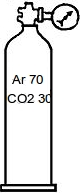
\includegraphics[width=.15\textwidth]{ballon.jpg}};
%		\draw[very thick] (1.2,2.5) -- (2,2.5);
%		\draw[very thick] (2.5,2.5) circle [radius=0.5];
%		\node[] at (2.5,2.5) {$\nearrow$};
		\draw[very thick] (3,2.5) -- (5.5,2.5);
		\draw[thick](4-.2,3) -- (4+.2,2) -- (4-.2,2) -- (4+.2,3) -- (4-.2,3);
		\node[below] at (4,2) {flowmeter1\footnote{flowmeter $V\ddot{o}gtim~V100$}};
		
		\draw (5.6,2.5) ellipse (.1 and .2);
		\draw (5.6,2.7)-- (8,2.7);
		\draw (8,2.5) ellipse (.1 and .2);
		\draw (8,2.3) -- (5.6,2.3);
		\node [below] at (6.6,2.3) {tube};
		
		\draw[very thick] (8,2.5) -- (11,2.5);
		
		\draw[thick](10-.2,3)--(10+.2,2)--(10-.2,2)--(10+.2,3)--(10-.2,3);
		\node[below] at (10,2) {flowmeter2};
		
		\draw[very thick] (8.5,2.5)--(8.5,.5);
		
		\draw(8.5,0) circle [radius=0.5];
		\node at (8.5,0) {P};
		\node[left] at (8,0) {pressuremeter};
		
		\draw[very thick] (11,2.5) -- (11,.5);
		\draw(11,0) circle [radius=0.5];
		\node at (11,0) {B};
		\node[below] at (11,-.5) {Bubbler};
		
		\draw[very thick] (11.5,0) -- (12.5,0) -- (12.5,1);
		\node[above] at (12.5,1) {atmosphere};
	\end{tikzpicture}
	\caption{Gas circulation scheme and circuit of connection of flow control through the drift tube}
	\label{fig:gasFlowScheme}
	\end{figure}		
	
	The electric scheme of the drift tube connection is shown in the Fig.\ref{fig:electricCircuit}.
	
%	Електронна схема підключення дрейфової трубки зображена на рис. \ref{fig:electricCircuit}.
	
	\tikzset{circuit declare symbol = ammeter}
	\tikzset{set ammeter graphic ={draw,generic circle IEC, minimum size=5mm, info=center:A}}

	\begin{figure}[!h]
	\begin{tikzpicture}[circuit ee IEC]
		\draw (0,0) rectangle (2,2);
		\node[left] at (2,0.5) {-};
		\node[left] at (2,1.5) {+};
		\node[] at (1,1) {HV};
		\draw (1.5,.5) to [ground={pos=1}] (1.5,-0.5);		
		
		\draw (2,1.5) to [resistor={ohm sloped=10M}] (6,1.5);
		\node [contact] at (2.5,1.5) {};
		\node [contact] at (6,1.5) {};
		
		\draw (2,0.5) to[ammeter] (6,.5);
		\node [contact] at (2.5,.5) {};
		\node [contact] at (4.5,.5) {};
		
%		\draw (5,.5) to [ground={pos=1}] (5,-0.5);
		
		\draw[very thick] (6,2.5) -- (10,2.5);
		\draw[very thick] (6,1.5) ellipse (0.3 and 1);
		\draw[very thick] (6,0.5) -- (10,0.5);
		\draw[very thick,shade] (10,1.5) ellipse (0.3 and 1);
		\draw[very thick, dashed, gray] (6,1.5) -- (10,1.5);
		
		\node [contact] at (10.5,1.5) {};
		\draw (10.3,1.5) to [capacitor={farad sloped=1n}] (11.5,1.5);
		
		\draw (12.5,1) node[op amp,yscale=-1] (opamp2) {};
		\draw (11.3,.5) to [ground={pos=1}] (11.3,-0.5);
		
%	amplifier with describing
%		\draw (3,0) node[op amp,yscale=-1] (opamp2) {}
%			(opamp2.+) node[left ] {$v_+$}
%  			(opamp2.-) node[left ] {$v_-$};
		
		\node [contact] at (13.7,1) {};
		\node[right] at (13.7,1) {Out};
	\end{tikzpicture}
	\caption{The electric scheme of the drift tube connection }
	%\caption{Електронна схема підключення тестового зразка дрейфової трубки}
	\label{fig:electricCircuit}	
	\end{figure}
	
	As it is seen above, the scheme is very simple.
	
	For our research we used a source $Fe^{55}$ which is suitable for a drift tube calibration. In our case $Fe^{55}$ serves as a photon source with almost monochromatic spectra with energy 5.9 keV.
	
	The most important parameter which we have to measure is Gain $G$ (\ref{eq:gain}).
	
	The idea is to measure a charge that goes through the tube electric circuit per unit of time and then find Gain.  We assume that a current $I_0$ through the ampere meter(see fig.~\ref{fig:electricCircuit}) is constant when the radioactive source is absent. The current  is non-zero when the tube detects background particles(for example atmospheric muon flux) or when  a leakage current is present. Therefore, with the presence of a source $Fe^{55}$ all surplus of the current $\bigtriangleup I = I-I_0$ in the drift tube circuit occurs because of gamma ray detection.
	
	On the other hand, we can write $\bigtriangleup I$ in terms of initial amount of electrons and Gain in the following form :
	
	\begin{equation}
	\bigtriangleup I = G N_0 e,
	\label{eq:IGainN0}
	\end{equation}
	
	where $G$ -- Gain; $N_0$ - number of initial electron-ion pairs per second; e - charge of electron in C.
	
	On the other hand we can express $N_0$ as:

	\begin{equation}
	N_0 = R \cdot \mean{n} = R \cdot\sum_n n p(n) \approx R \int_0^\infty n p(n) dn;
	\end{equation}

	where  $p(n)$ is a probability that the photon with energy 5.9 keV after interaction with argon atom will create $n$ electron-ion pairs; R is a rate [Hz], as we need to find the amount of electron-ion pairs per one second.

	The calculation of the distribution 	$p(n)$  in GARFIELD is shown in Fig.\ref{fig:n_probability}. In the figure we can the two peaks: the main photopeak and the smaller escape peak. 
%	Тут $p(n)$ - імовірність того, що фотон з енергією 5.9 КеВ провзаємодівши з атомом аргону утворить $n$ електрон іонних пар, R - частоса реєстрації сигналів [Hz] так як нам потрібно знайти кількість електрон-іонних пар за час 1с.	
%	Розрахунок розподілу $p(n)$ в GARFIELD подано на рисунку \ref{fig:n_probability}. Як видно з рисунку в розподілі $p(n)$ присутньо 2 піки: основний фотопік, та менший escape peak. 
	The escape peak for argon is known to be 3.2 keV less than the primary peak. An escape peak is formed by a number of photon interactions in the gas resulting in one primary ionization electron and a re-emitted X-ray with a long mean free path.
	
	\begin{figure}[!h]
	\centering
	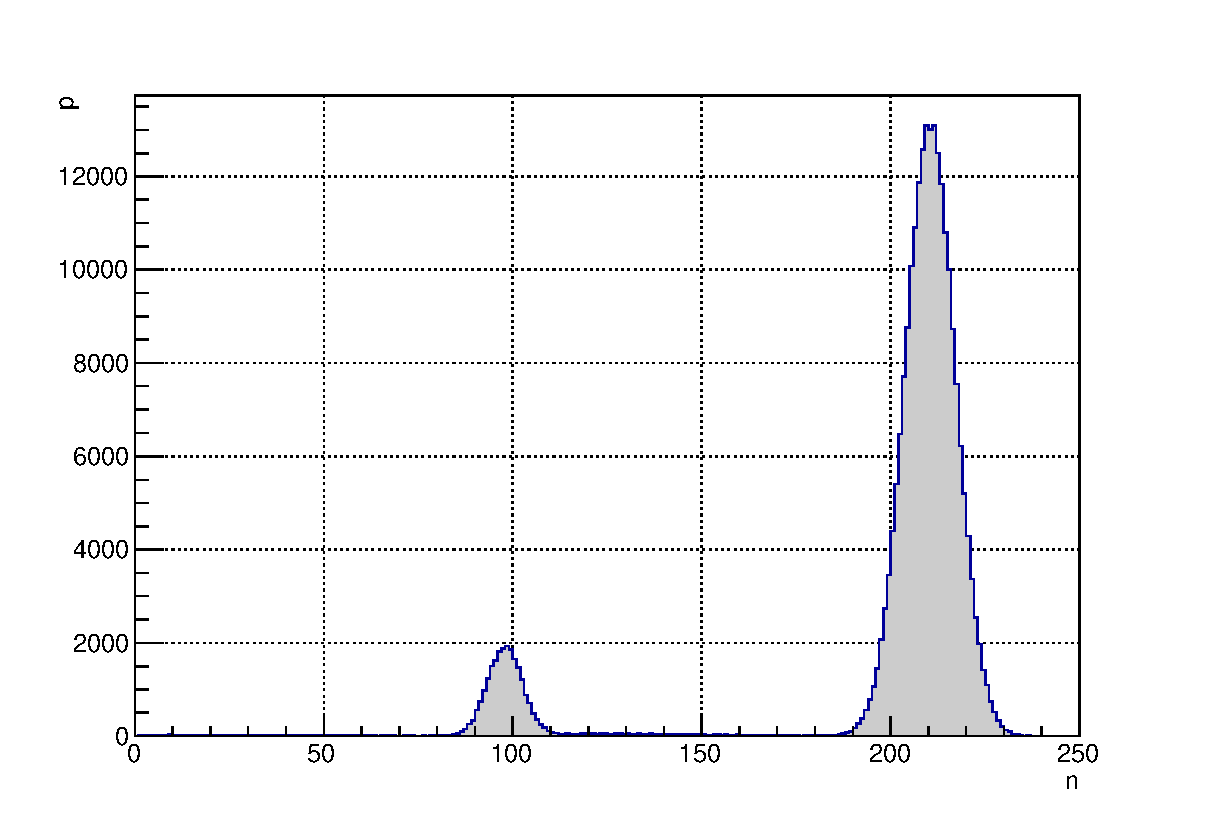
\includegraphics[width=0.7\textwidth]{fe55neGamma}
	\caption{ p(n) distribution}
%	\caption{ Розподіл актів взаємодії фотонів енергії 5.9 кеВ з газом Аргону від кількості первинних електронів, утворених в об’ємі дрейфової трубки}
	\label{fig:fe55_n_probability}
	\end{figure}
	
	The realisation of a measurement is very simple.  On the amplifier output (see Fig.\ref{fig:electricCircuit}) the signal goes to the discriminator with  trigger threshold on the level enough for a signal detection and big enough for noise neglecting. The signal from discriminator in rectangular form goes into counter. The counter is triggered for the rising edge. This scheme has a small dead time $~0.5 \mu s$, therefore for the signal frequency of $R \sim 5000 \frac{events}{second} \approx 200 \frac{\mu s}{event}$ the amount of non counted signals is negligibly small.
	
	For the first gain estimation we assume about avalanche superposition and linear amplitude dependence of final signal on the amount of initial electrons(later we will show that this is not true).
	
	From the distribution in Fig.\ref{fig:fe55_n_probability} we can find $\mean{n} = 197.87$ for average amount of primary electron because of photon (5.9keV) interaction with atoms of a gas $Ar70\%+CO_230\%$.
	
	The results of measurements are shown in the table \ref{table:GainTotal}. The Gain curves G(V) for several pressure values are shown in the Fig.\ref{fig:Gain_multy}.
		
%	Постановка експерименту виглядає досить примітивно. На виході з підсилювача (див рис.\ref{fig:electricCircuit}) сигнал подається на дискримінатор з порогом спрацьовування виставленим на рівні достатньому для реєтрації сигналів але достньо високим, щоб шум не зараховувався. Сигнал з дискримінатора у вигляді прямокутного сигналу подається на лічильних, який спрацьовує по зростаючому фронту. Така схема має малий мертвий час порядку $0.5 \mu s$, тому для частоти сигналів $R \sim 5000 \frac{events}{second} \approx 200 \frac{\mu s}{event}$ кількість незарахованих сигналів буде нищівно мала.
	
%	Для першої оцінки коефіцієнту підсилення ми припускаємо про таку собі суперпозицію лавин і лінійну маштабованість амплітуди кінцевого сигналу від кількості початкових електронів(далі ми покажемо що це не так).
	
%	З розподілу на рис.\ref{fig:fe55_n_probability} знаходимо $\mean{n} = 197.87$ для середньої кількість первинних електронів від акту взаємодії фотону енергії $5.9 keV$ з атомами газу  $Ar70\%+CO_230\%$.
	
%	Результати вимірювань представимо у вигляді таблиці \ref{table:GainTotal}. Криві коефіцієнту підсилення G(V) для ряду значень тиску зображено на рис.
	
%	Для обрахунку сигналу спершу розглянемо специфіку взамодії гамма-квантів з енергією 5.9 КеВ з Аргоном.
	
	\begin{table}[!h]
	\centering
	\begin{tabular}{|l|l|l|l|l|l|l|}
		\hline
		Gain(no cor) & P[bar] (U[V]) & HV [V] & Thr [mV]&  I [nA] & RMS [nA] & Rate [Hz]  \\
		\hline
		11138 & 1.0(0.857) & 1600 & &  1.7700 & 0.0919 & = \\
		\hline
		18196 & 1.0(0.857) & 1650 & &  2.8915 & 0.1598 & = \\
		\hline
		29255 & 1.0(0.857) & 1700 & 32 & 4.6490 & 0.2328 & 4965.9 \\
		\hline
		47012 & 1.0(0.858) & 1750 & & 7.4707 & 0.4380 & = \\
		\hline
		73159 & 1.0(0.857) & 1800 & & 11.6257 & 0.5630 & = \\
		\hline
		
		& & & & & & \\
		\hline
		
		9885 & 1.106(0.906) & 1650 & & 1.6921 & 0.1099 & = \\
		\hline
		15747 & 1.106(0.905)& 1700 & & 2.6955 & 0.13381 & = \\
		\hline
		25275 & 1.106(0.905)& 1750 & 32 & 4.3263 & 0.1975 & 5349.0 \\
		\hline
		39887 & 1.106(0.906)& 1800 & & 6.8274 & 0.2841 & = \\
		\hline
		61359 & 1.106(0.906)& 1850 & & 10.5028 & 0.4567 & = \\
		\hline
		
		& & & & & & \\
		\hline
		
		9260 & 1.205(0.951) & 1700  & & 1.6921 & 0.1053 & \\
		\hline
		14536 & 1.205(0.951) & 1750 & & 2.6562 & 0.1274 & \\
		\hline
		22991 & 1.205(0.951) & 1800 & 32 & 4.2012 & 0.1900 & 5710 \\
		\hline
		35777 & 1.205(0.951) & 1850 & & 6.5376 & 0.2880 & \\
		\hline
		54684 & 1.205(0.951) & 1900 & & 9.9924 & 0.5284 & \\
		\hline
		
		& & & & & & \\
		\hline
		
		5444 & 1.309 (0.998) & 1700 &  & $1.03 $ & $ 0.06 $ & \\
		\hline
		8351 & 1.309 (0.998) & 1750 &  & $1.58 $ & $ 0.14$ & \\
		\hline
		13267 & 1.309 (0.998) & 1800 &  & $2.51 $ & $ 0.12 $ & \\
		\hline
		20615 & 1.309 (0.998) & 1850 & 32 & $3.90 $ & $ 0.15 $ & 5987 \\
		\hline
		31716 & 1.309 (0.998) & 1900 &  & $6.00 $ & $ 0.29 $ & \\
		\hline
		48102 & 1.309 (0.998) & 1950 &  & $9.10 $ & $ 0.38 $ & \\
		\hline
		69987 & 1.309 (0.998) & 2000 &  & $13.24 $ & $ 0.50 $ & \\
		\hline
		100751 & 1.309 (0.998) & 2050 &  & $19.06 $ & $ 0.78 $ & \\
		\hline
		
	\end{tabular}
	\caption{Gain measurements}
%	\caption{Виміри коефіцієнту підсилення трубки}
	\label{table:GainTotal}
	\end{table}
	
	\begin{figure}[!h]
	\centering
	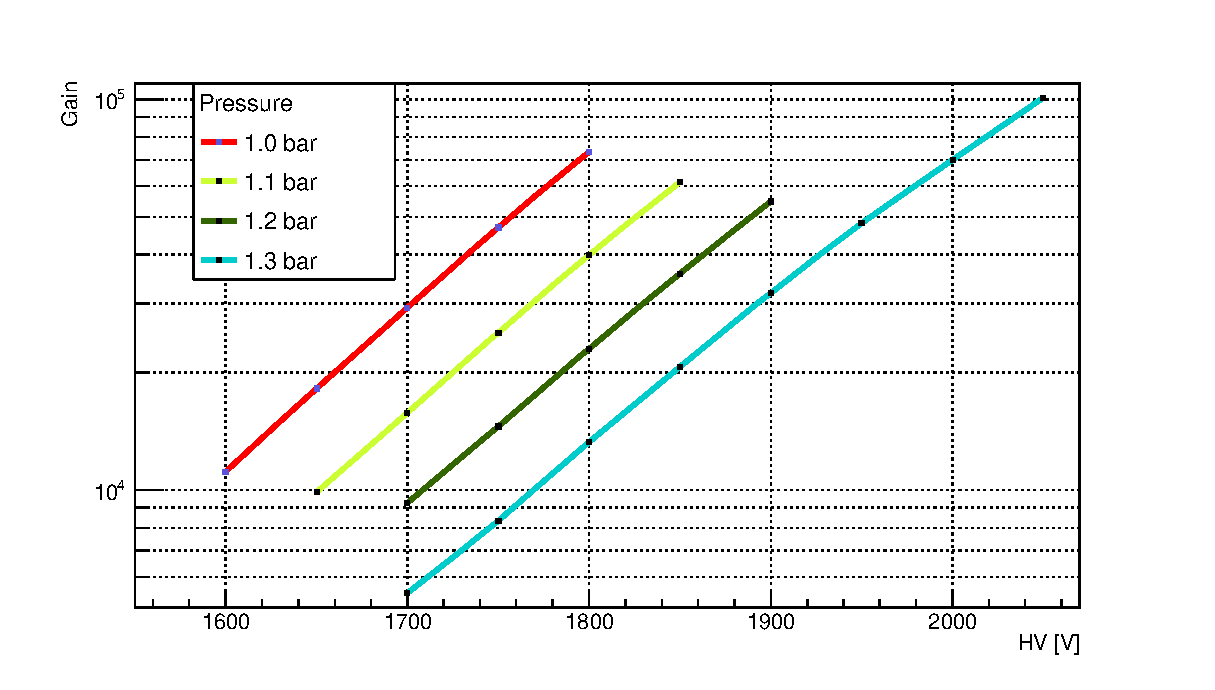
\includegraphics[width=1.0\textwidth]{gain_multyGraph}
	\caption{Gain experimental curves for several values of gas pressure in the drift tube.}
%	\caption{ Експериментальні криві коефіцієнту підсилення для набору значень тиску в дрейфовій трубці}
	\label{fig:Gain_multy}
	\end{figure}
		
	
	\subsection{Experimental spectra from the source Fe55}
		
	$^{55}Fe$  is a source of gamma-rays with energy of 5.9 keV. Each signal at the output of amplifier differs by amplitude in dependence of initial electron number. Therefore, according to the calculated in GARFIELD spectra $p(n)$ (see Fig.\ref{fig:fe55_n_probability}), it is expected to see two peaks in experimental spectra.
	
	For spectra measurements we first have to get a match between a certain signal and the amplitude on the output of the drift tube. In our case such a quantity is an integral from a signal on during the time of a signal.
	
	The amplified signal from the output of the amplifier is sent in parallel through the linear splitter to the discriminator and delay system. With the signal from discriminator the sampling signal and busy signal is formed. During the busy signal the analysing system does not accept the signal from the drift tube (this is a dead time for this detector system). The delayed signal from the amplifier integrates during the sampling signal and then digitalizes with 10-bit ADC. After digitalizing the signal is sent through the optical channel to PC, where the data is recorded into separate ROOT-file.
	
	The stages {\it sampling + storing} are time-consuming and a dead time in this case is bigger than an average time interval between events in the tube(with current detector system) therefore is a big probability to miss detecting an event.
	
	The sampling stage is built in such a way to calibrate for pedestal shelf voltage from the integrator. On the final histogram it will look as a small peak. We will calibrate exactly with regard to it. The second control point is a gamma-ray 5.9 keV photo peak from the source $^{55}Fe$.
	
	\begin{figure}
	\centering
	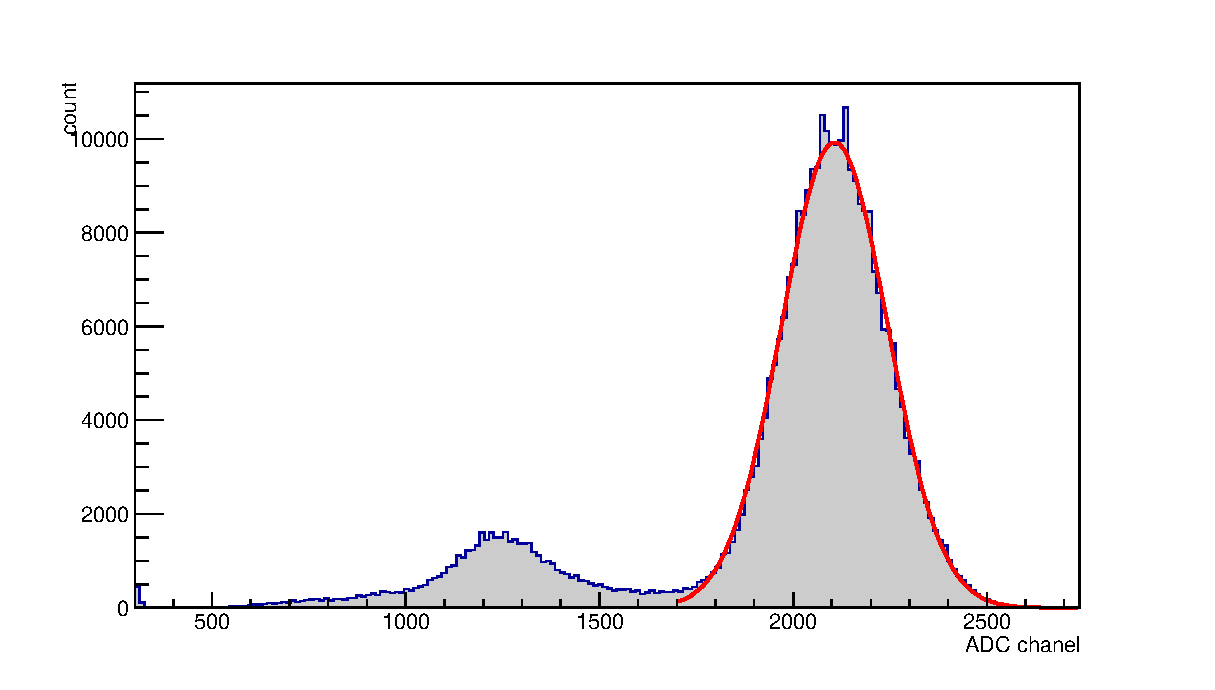
\includegraphics[width=0.7\textwidth]{expFitted1750}
	
	\caption{Experimental spectra from $^{55}Fe$.}
	\label{fig:expFitted1750}
	\end{figure}
	
%	$Fe^{55}$ - по суті є джерелом гама-квантів з енергією 5.9 КеВ. На практиці  очікуємо побачити 2 піки відповідно до симуляції(дивись рис. \ref{fig:fe55_n_probability}).
	
%	Для того, щоб вести мову про спектр спершу необхідно кожному сигналу привести у відповідність число яке лінійно залежало би від амплітуди сигналу на виході з трубки. В нашому випадку такою величиною є інтеграл від сигналу вздовж часу порядку протяжності сигналу.
	
%	Підсилений сигнал на виході з підсилювача через через лінійний розгалуджувач  паралельно пускається на дискримінатор та систему затримки. З сигналу від дискримінатора формує сигнал для вибірки сигналу, а також сигнал busy, впродовж якого аналізуча система не приймає сигнал(по суті це є мертвим часом даної детекторної установки). Затриманий сигнал від підсилювача інтегрується протягомі sampling signal і оцифровуєтсья 10 бітним АЦП. Оцифрований сигнал через оптичний канал посилається на ПК де дані гістограмуються в окремий root-файл.
	
%	Процес sampling + storing досить часо затратний, і мертвий час в даному випадку є більший за середню відстань між подіями в трубці, тому є велика імовірність пропустити події.
	
%	Етап самплінгу побудований таким чином, що дозволяє відкалібрувати сигнал для випадку відсутності сигналу в трубці. На кінцевій гістограмі це виливаєтсья в маленький пік. Відносно нього ми і будемо калібруватися. Другою реперною точкою в нас буде фотопік від gamma квантів 5.9 КеВ джерела $Fe^{55}$.
	
	\begin{table}[!h]
	\centering
	\begin{tabular}{|l|r|l|}
		\hline
		point of reference & channel & electrons per cluster(simulations)\\
		\hline
		zero pedestal ($gauss~\mu \pm \bigtriangleup \mu)$ & $301.1 \pm 0.3 $ & 0\\
		\hline
		$5.9~keV$ & $2107.4 \pm 0.3$ & $210.42 \pm 0.01$ \\ 
		\hline
		escape peak & $1253.3 \pm 0.9 $ & $97.99 \pm 0.03$ \\
		\hline
	\end{tabular}
	\caption{ Coordinates of peaks from Fig.\ref{fig:expFitted1750} and Fig.\ref{fig:fe55_n_probability}}
%	\caption{ Координати центрів піків на симуляціях(в одиницях кількості електронів на подію) та спектр зі спектрометра (вихід 12 бітного АЦП)}
	\label{table:peakPos}
	\end{table}
	
	\subsection{ Space charge effect}
	
	Photons from $^{55}Fe$ of energy 5.9 keV create $\sim 200$ electron-ion pairs as a result of photoeffect with $Ar70\%+CO_230\%$ gas mixture. As we have a strong electric field between anode and cathode such electron cloud starts to drift toward a wire. The external field distorts as any space charge creates its own e/m field. As a result, partial avalanches per initial electron of a cloud creates an avalanche of size smaller than from a single-electron cloud(as in case muon ionisation).
	
	Such an effect indeed was observed. If we suppose a linear dependence of output signal amplitude from number of initial electrons a relative position for experimental peak should be located at(calibration relatively to the photopeak):
	
	\begin{equation}
			channel_{escapePeak} = \frac{2107.4 - 301.1}{210.42} 98 + 301.1 = 1142.3 \ne 1253.3,
	\end{equation}
